% Build from this directory:
% latex -interaction=nonstopmode -halt-on-error pam-3.tex
% dvisvgm --no-fonts --exact --bbox=papersize pam-3.dvi -o pam-3.svg
\documentclass[tikz,border=4pt]{standalone}
\definecolor{equalblue}{HTML}{4472C4}
\definecolor{equalorange}{HTML}{ED7D31}
\definecolor{cellborder}{HTML}{2F528F}
\begin{document}
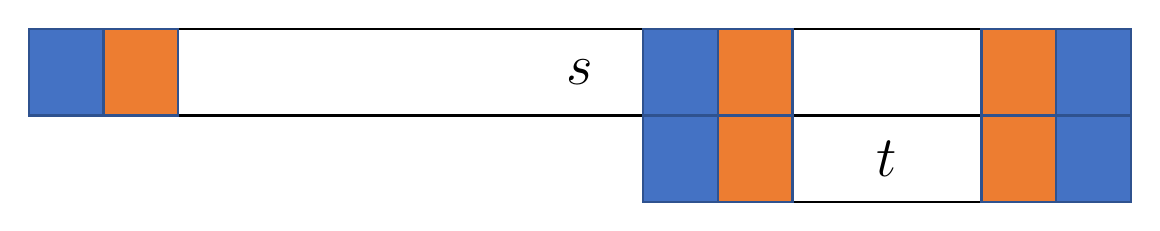
\begin{tikzpicture}[line width=0.8pt,font=\fontsize{20}{24}\selectfont]
  % The lower row is the suffix t of s. Equal colors mark equal characters.
  \draw[fill=white] (0,0) rectangle (14,1.1);
  \draw[fill=white] (7.8,-1.1) rectangle (14,0);
  \foreach \left/\right/\shade in {
    0/0.95/equalblue,0.95/1.9/equalorange,
    7.8/8.75/equalblue,8.75/9.7/equalorange,
    12.1/13.05/equalorange,13.05/14/equalblue} {
    \draw[draw=cellborder,fill=\shade] (\left,0) rectangle (\right,1.1);
  }
  \foreach \left/\right/\shade in {
    7.8/8.75/equalblue,8.75/9.7/equalorange,
    12.1/13.05/equalorange,13.05/14/equalblue} {
    \draw[draw=cellborder,fill=\shade] (\left,-1.1) rectangle (\right,0);
  }
  \node at (7,0.55) {$s$};
  \node at (10.9,-0.55) {$t$};
\end{tikzpicture}
\end{document}
